\documentclass{standalone}
\usepackage{tikz}
\usetikzlibrary{patterns, positioning}
\usetikzlibrary{shapes.misc}
\usepackage[outline]{contour}
\contourlength{1.5pt} 


\begin{document}
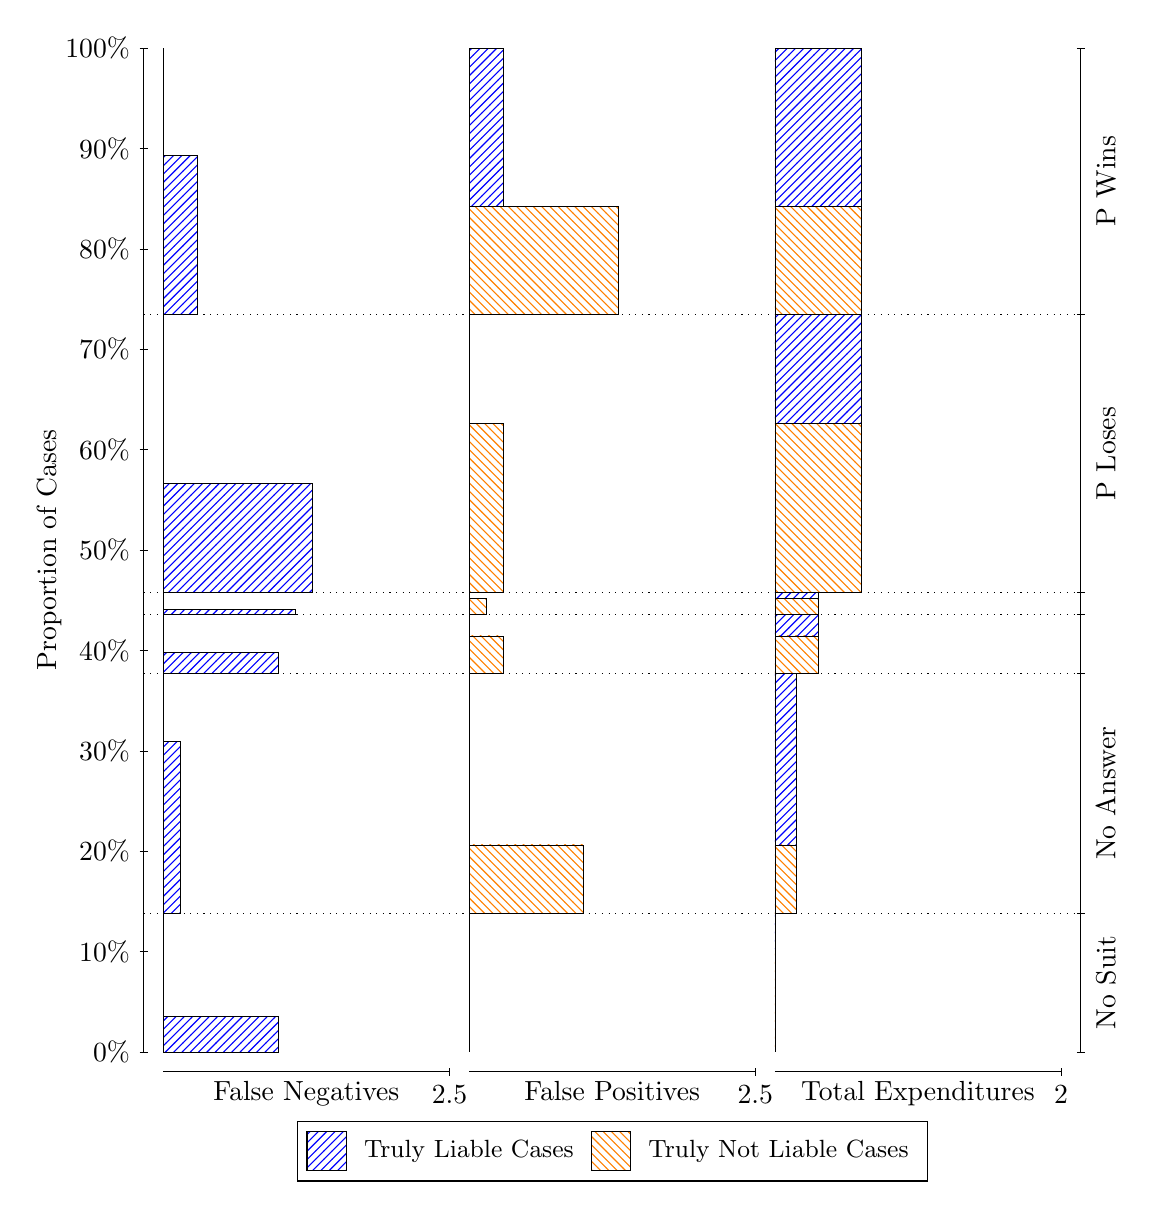
\begin{tikzpicture}
\draw[black, very thin] (1.5,1.75) -- (1.5,14.5);
\node[rotate=90, text=black, anchor=center] at (0.3, 8.125) {Proportion of Cases};
\draw[black, very thin] (1.45,1.75) -- (1.55,1.75);
\node[text=black, anchor=east] at (1.45, 1.75) {0\%};
\draw[black, very thin] (1.45,3.025) -- (1.55,3.025);
\node[text=black, anchor=east] at (1.45, 3.025) {10\%};
\draw[black, very thin] (1.45,4.3) -- (1.55,4.3);
\node[text=black, anchor=east] at (1.45, 4.3) {20\%};
\draw[black, very thin] (1.45,5.575) -- (1.55,5.575);
\node[text=black, anchor=east] at (1.45, 5.575) {30\%};
\draw[black, very thin] (1.45,6.85) -- (1.55,6.85);
\node[text=black, anchor=east] at (1.45, 6.85) {40\%};
\draw[black, very thin] (1.45,8.125) -- (1.55,8.125);
\node[text=black, anchor=east] at (1.45, 8.125) {50\%};
\draw[black, very thin] (1.45,9.4) -- (1.55,9.4);
\node[text=black, anchor=east] at (1.45, 9.4) {60\%};
\draw[black, very thin] (1.45,10.675) -- (1.55,10.675);
\node[text=black, anchor=east] at (1.45, 10.675) {70\%};
\draw[black, very thin] (1.45,11.95) -- (1.55,11.95);
\node[text=black, anchor=east] at (1.45, 11.95) {80\%};
\draw[black, very thin] (1.45,13.225) -- (1.55,13.225);
\node[text=black, anchor=east] at (1.45, 13.225) {90\%};
\draw[black, very thin] (1.45,14.5) -- (1.55,14.5);
\node[text=black, anchor=east] at (1.45, 14.5) {100\%};

\draw[black, very thin] (13.4,1.75) -- (13.4,14.5);
\draw[black, very thin] (13.35,1.75) -- (13.45,1.75);
\node[anchor=west] at (13.35, 1.75) {};
\draw[black, very thin] (13.35,3.5135) -- (13.45,3.5135);
\node[anchor=west] at (13.35, 3.5135) {};
\draw[black, very thin] (13.35,6.5578) -- (13.45,6.5578);
\node[anchor=west] at (13.35, 6.5578) {};
\draw[black, very thin] (13.35,7.304) -- (13.45,7.304);
\node[anchor=west] at (13.35, 7.304) {};
\draw[black, very thin] (13.35,7.5819) -- (13.45,7.5819);
\node[anchor=west] at (13.35, 7.5819) {};
\draw[black, very thin] (13.35,11.12) -- (13.45,11.12);
\node[anchor=west] at (13.35, 11.12) {};
\draw[black, very thin] (13.35,14.5) -- (13.45,14.5);
\node[anchor=west] at (13.35, 14.5) {};

\draw[black, very thin, pattern color=blue, pattern=north east lines] (1.75,1.75) rectangle (3.2033,2.2065);
\draw[black, very thin, pattern color=orange, pattern=north west lines] (1.75,2.2065) rectangle (1.75,3.5135);
\draw[black, very thin, pattern color=blue, pattern=north east lines] (1.75,3.5135) rectangle (1.968,5.6901);
\draw[black, very thin, pattern color=orange, pattern=north west lines] (1.75,5.6901) rectangle (1.75,6.5578);
\draw[black, very thin, pattern color=blue, pattern=north east lines] (1.75,6.5578) rectangle (3.2033,6.8289);
\draw[black, very thin, pattern color=orange, pattern=north west lines] (1.75,6.8289) rectangle (1.75,7.304);
\draw[black, very thin, pattern color=blue, pattern=north east lines] (1.75,7.304) rectangle (3.4213,7.3726);
\draw[black, very thin, pattern color=orange, pattern=north west lines] (1.75,7.3726) rectangle (1.75,7.5819);
\draw[black, very thin, pattern color=blue, pattern=north east lines] (1.75,7.5819) rectangle (3.6393,8.9677);
\draw[black, very thin, pattern color=orange, pattern=north west lines] (1.75,8.9677) rectangle (1.75,11.12);
\draw[black, very thin, pattern color=blue, pattern=north east lines] (1.75,11.12) rectangle (2.186,13.136);
\draw[black, very thin, pattern color=orange, pattern=north west lines] (1.75,13.136) rectangle (1.75,14.5);
\draw[black, very thin, pattern color=orange, pattern=north west lines] (5.6333,1.75) rectangle (5.6333,3.057);
\draw[black, very thin, pattern color=blue, pattern=north east lines] (5.6333,3.057) rectangle (5.6333,3.5135);
\draw[black, very thin, pattern color=orange, pattern=north west lines] (5.6333,3.5135) rectangle (7.0867,4.3812);
\draw[black, very thin, pattern color=blue, pattern=north east lines] (5.6333,4.3812) rectangle (5.6333,6.5578);
\draw[black, very thin, pattern color=orange, pattern=north west lines] (5.6333,6.5578) rectangle (6.0693,7.0329);
\draw[black, very thin, pattern color=blue, pattern=north east lines] (5.6333,7.0329) rectangle (5.6333,7.304);
\draw[black, very thin, pattern color=orange, pattern=north west lines] (5.6333,7.304) rectangle (5.8513,7.5133);
\draw[black, very thin, pattern color=blue, pattern=north east lines] (5.6333,7.5133) rectangle (5.6333,7.5819);
\draw[black, very thin, pattern color=orange, pattern=north west lines] (5.6333,7.5819) rectangle (6.0693,9.734);
\draw[black, very thin, pattern color=blue, pattern=north east lines] (5.6333,9.734) rectangle (5.6333,11.12);
\draw[black, very thin, pattern color=orange, pattern=north west lines] (5.6333,11.12) rectangle (7.5227,12.484);
\draw[black, very thin, pattern color=blue, pattern=north east lines] (5.6333,12.484) rectangle (6.0693,14.5);
\draw[black, very thin, pattern color=orange, pattern=north west lines] (9.5167,1.75) rectangle (9.5167,3.057);
\draw[black, very thin, pattern color=blue, pattern=north east lines] (9.5167,3.057) rectangle (9.5167,3.5135);
\draw[black, very thin, pattern color=orange, pattern=north west lines] (9.5167,3.5135) rectangle (9.7892,4.3812);
\draw[black, very thin, pattern color=blue, pattern=north east lines] (9.5167,4.3812) rectangle (9.7892,6.5578);
\draw[black, very thin, pattern color=orange, pattern=north west lines] (9.5167,6.5578) rectangle (10.062,7.0329);
\draw[black, very thin, pattern color=blue, pattern=north east lines] (9.5167,7.0329) rectangle (10.062,7.304);
\draw[black, very thin, pattern color=orange, pattern=north west lines] (9.5167,7.304) rectangle (10.062,7.5133);
\draw[black, very thin, pattern color=blue, pattern=north east lines] (9.5167,7.5133) rectangle (10.062,7.5819);
\draw[black, very thin, pattern color=orange, pattern=north west lines] (9.5167,7.5819) rectangle (10.607,9.734);
\draw[black, very thin, pattern color=blue, pattern=north east lines] (9.5167,9.734) rectangle (10.607,11.12);
\draw[black, very thin, pattern color=orange, pattern=north west lines] (9.5167,11.12) rectangle (10.607,12.484);
\draw[black, very thin, pattern color=blue, pattern=north east lines] (9.5167,12.484) rectangle (10.607,14.5);
\draw[black, dotted] (1.5,3.5135) -- (13.4,3.5135);
\draw[black, dotted] (1.5,6.5578) -- (13.4,6.5578);
\draw[black, dotted] (1.5,7.304) -- (13.4,7.304);
\draw[black, dotted] (1.5,7.5819) -- (13.4,7.5819);
\draw[black, dotted] (1.5,11.12) -- (13.4,11.12);
\draw[black, very thin] (1.75,1.5) -- (5.3833,1.5);
\node[text=black, anchor=north] at (3.5667, 1.5) {False Negatives};
\draw[black, very thin] (5.3833,1.45) -- (5.3833,1.55);
\node[text=black, anchor=north] at (5.3833, 1.45) {2.5};

\draw[black, very thin] (5.6333,1.5) -- (9.2667,1.5);
\node[text=black, anchor=north] at (7.45, 1.5) {False Positives};
\draw[black, very thin] (9.2667,1.45) -- (9.2667,1.55);
\node[text=black, anchor=north] at (9.2667, 1.45) {2.5};

\draw[black, very thin] (9.5167,1.5) -- (13.15,1.5);
\node[text=black, anchor=north] at (11.333, 1.5) {Total Expenditures};
\draw[black, very thin] (13.15,1.45) -- (13.15,1.55);
\node[text=black, anchor=north] at (13.15, 1.45) {2};

\node[text=black, centered, rotate=90] at (13.72, 2.6317) {\contour{white}{No Suit}};
\node[text=black, centered, rotate=90] at (13.72, 5.0356) {\contour{white}{No Answer}};


\node[text=black, centered, rotate=90] at (13.72, 9.3508) {\contour{white}{P Loses}};
\node[text=black, centered, rotate=90] at (13.72, 12.81) {\contour{white}{P Wins}};

\draw (7.449999999999999,1.5) node[draw=none] (baseCoordinate) {};
\begin{scope}[align=center]
        \matrix[scale=0.5, draw=black, below=0.5cm of baseCoordinate, nodes={draw}, column sep=0.1cm]{
            \node[rectangle, draw, minimum width=0.5cm, minimum height=0.5cm, pattern color=blue, pattern=north east lines] {}; &
            \node[draw=none, font=\small, text=black] (B) {Truly Liable Cases}; &
            \node[rectangle, draw, minimum width=0.5cm, minimum height=0.5cm, pattern color=orange, pattern=north west lines] {}; &
            \node[draw=none, font=\small, text=black] (B) {Truly Not Liable Cases}; \\
            };
\end{scope}

\end{tikzpicture}
\end{document}